\subsection{Grundlagen der schliessenden Statistik}
\begin{figure}[H]
	\centering
	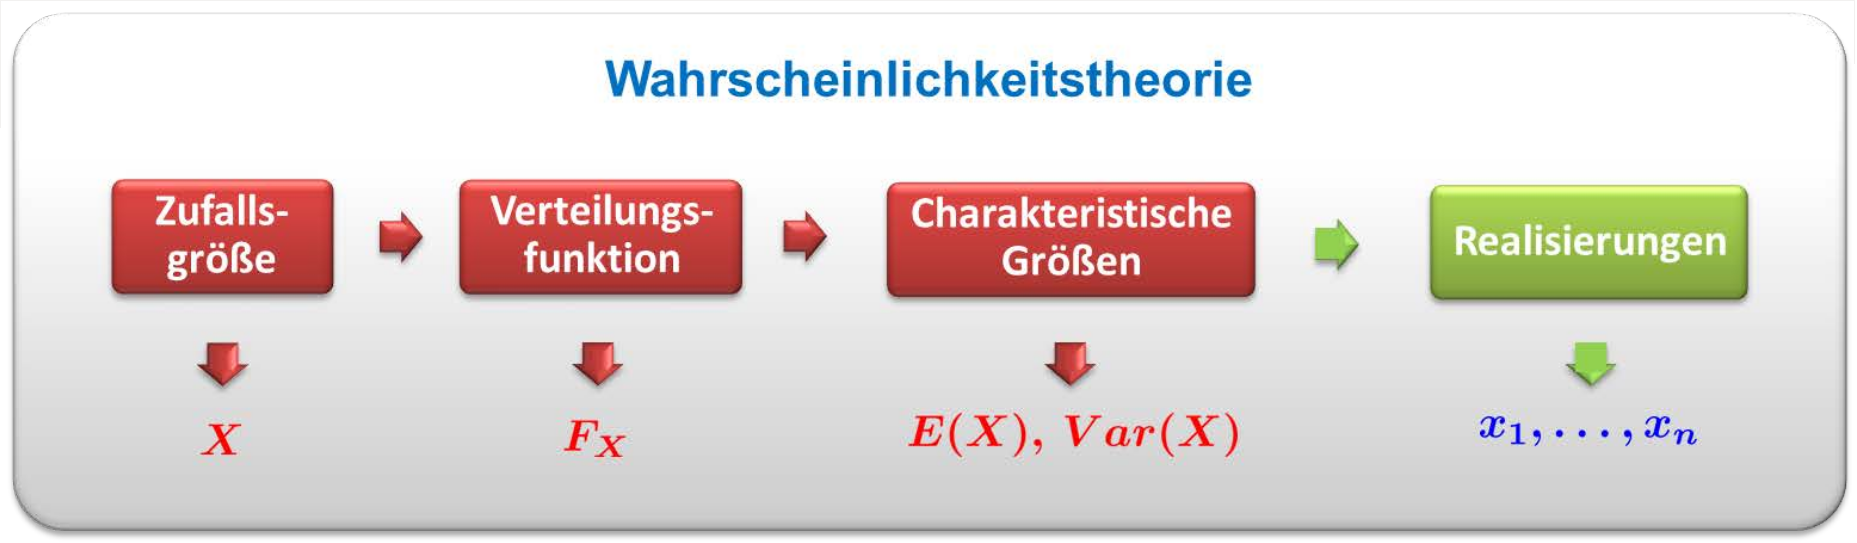
\includegraphics[scale=0.2]{images/exev_wahrscheinlichkeitstheorie.png}
	\caption{Wahrscheinlichkeitstheorie}
	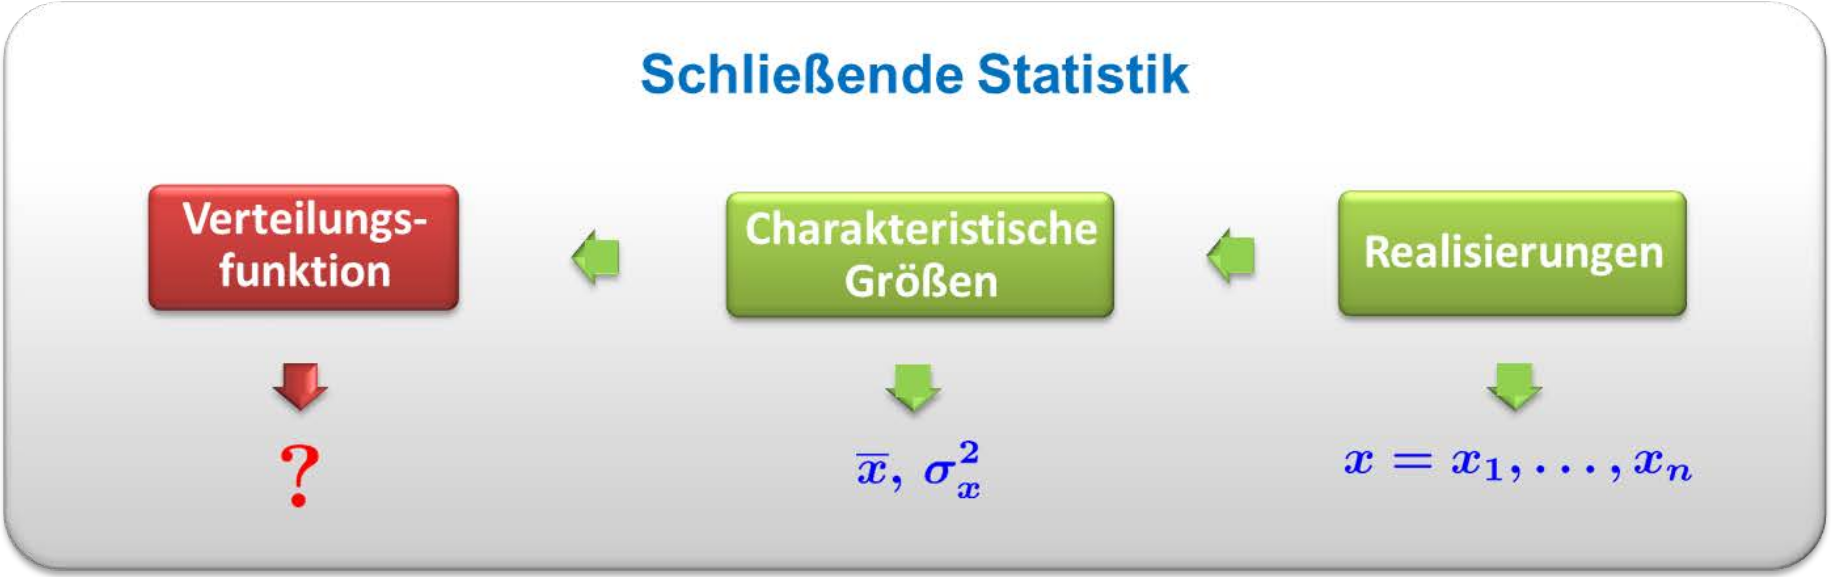
\includegraphics[scale=0.2]{images/exev_schliessende-statistik.png}
	\caption{Schliessende Statistik}
\end{figure}
\begin{tcolorbox}[colback=green!5,colframe=green!40!black,title=Wahrscheinlichkeitstheorie]
Die Wahrscheinlichkeitstheorie untersucht Grössen die vom Zufall beeinflusst werden. Die Art des Zufallseinflusses wird durch die spezielle Wahl der Verteilungsfunktion bestimmt. Mittels rein mathematiscner Überlegungen lassen sich bezüglich solcher Grössen bestimmte charakteristische Eigenschaften ableiten, welche schliesslich Rückschlüsse auf die Eigenschaften von Realisierungen solcher Grössen zulassen.
\end{tcolorbox}
Die schliessende Statistik befasst sich mit Messreihen deren konkrete Ausprägung vom Zufall beeinflusst werden. Diese Messreihen können ebenfalls charakteristische Grössen etwa in Form des arithmetischen Mittels und der Varianz zugeordnet werden. Hier stellt sich die Frage nach der Gestalt des unbekannten Verteilungsgesetzes unter dem die vorliegende Realisierung zustande kam. Eine Entscheidung über die Annahme oder Ablehnung einer angenommenen Verteilung kann durch ein Vergleich der gemessenen charakteristischen Grössen der Realisierung und aus der Theorie abgeleiteten charakteristischen Grössen des hypothetischen Verteilungsgesetzes getroffen werden.
\pagebreak[2]
\subsubsection{Stichprobenerhebung}
\begin{itemize}
	\item Einfache Zufallsstichprobe
	\item Geschichtete Stichprobe
	\item Klumpenstichprobe
	\item Systematische Stichprobe
	\item Mehrstufige Stichprobe
\end{itemize}
Um gut Stichproben zu erheben muss man folgende Punkte beachten
\begin{enumerate}
\item Im Rahmen der Datenerhebung
\subitem Isolierende Abstraktion\\
Hier sind die unterschiedlichen Eigenschaften der Stichprobenerhebung zu beachten. Das passende Verfahren hängt stark von der Fragestellung und dem zu untersuchenden Objekt bzw. System ab, die durch die Simulation beantwortet werden soll. Um signifikante Aussagen machen zu können, ist die Grösse der Stichprobe zu bestimmen.
\subitem Generalisierende Abstraktion\\
Es muss eine geeignete Verteilungsfunktion gefunden werden, um die Anzahl der möglichen Experimente zu erhöhen und eine gewisse Variabilität zu ermöglichen.
\item Im Rahmen der Experimentauswertung
\subitem Festlegung der Verteilung der Eingangsdaten\\
% TODO: Überarbeiten
Sind diese festgelegt folgen die Experimente. Sind die Verteilungen zufällig, so kann diese nur durch die Festlegung eines Seeds bestimmt werden, sodass sich die Streuung um einen Mittelwert ergibt. Wurden die Eingangsdaten falsch bestimmt, wird in den folgenden Experimenten ein systematischer Fehler gemacht, der zu falschen Rückschlüssen führt
\subitem Für die Experimentplanung und Auswertung ergeben sich folgende Fragen:
\pagebreak[2]
\begin{itemize}
\item Wie sieht die Stichprobenfunktion und ihre Wahrscheinlichkeitsverteilung aus?
\item Wie kann ein Vertrauensintervall für den Mittelwert bzw. die Varianz einer Messreihe ermittelt werden?
\item Wie kann der Stichprobenumfang d.h. die Anzahl der Experimente, festgelegt werden?
\item Welche etablierten Testverfahren gibt es?
\end{itemize}
\end{enumerate}
\begin{tcolorbox}[colback=green!5,colframe=green!40!black,title=Testverteilungen]
Testverteilungen sind Verteilungen, die bei vielen statistischen Tests Verwendung finden. Wichtige Testverteilungen sind
\begin{itemize}
\item Chi-Quadrat Verteilung (\autoref{theorie:chiquadrat})
\item $t$-Verteilung (auch Student $t$-Verteilung) wenn die Stichprobe $<30$ ist (\autoref{theorie:t_verteilung})
\item Normalverteilung wenn die Stichprobe $\leq 30$ ist (\autoref{theorie:normalverteilung})
\end{itemize}
\end{tcolorbox}
%---------------------------------------------------------------------
\pagebreak[2]
\subsection{Chi-Quadrat Verteilung}\label{theorie:chiquadrat}
Dies ist eine stetige Wahrscheinlichkeitsverteilung über der Menge der positiven reellen Zahlen. Ihr einziger Parameter muss eine natürliche Zahl sein und wird Freiheitsgrad genannt. Sie ist eine der Verteilungen, die aus der Normalverteilung abgeleitet werden könne. Ha man Zufalls-variablen, die unabhängig und standardorientiert sind, so ist die Chi-Quadrat Verteilung mit Freiheitsgraden definiert als die Verteilung der Summe der quadrierten Zufalls-variablen. Solche Summen quadrierter Zufalls-variablen treten bei der Schätzung der Varianz einer Stichprobe auf.\\
Dichte der $\chi_r^2$-Verteilung mit $r$ Freiheitsgraden:
\begin{equation}\label{eq:chisqare:1}
f(t)=\left\{\begin{array}{l l} \frac{1}{2^{\frac{r}{2}}\Gamma(\frac{r}{2})}\cdot t^{\frac{r}{2}-1}\cdot e^{-\frac{t}{2}}&, \mbox{für }t > 0 \\ 0 &, \mbox{für } t \leq 0\end{array}\right.
\end{equation}
%Bild Chi Verteilung
Erwartungswert:
\begin{equation}
E(X) = r
\end{equation}
Varianz:
\begin{equation}
Var(X) = 2r
\end{equation}
%-------------------------------------------------------------------------
\subsection{Dichte der t-Verteilung}\label{theorie:t_verteilung}
Dichte der $t_r$-Verteilung mit $r$ Freiheitsgraden:
\begin{equation}
f(t)=\frac{1}{\sqrt{r}\cdot B(\frac{1}{2},\frac{r}{2})}\cdot (1+\frac{t^2}{r})^{-\frac{1}{2}(r+1)}\, , t\in\mathbb{R}
\end{equation}
Erwartungswert:
\begin{equation}
E(X) = 0 (\mbox{für }r > 1)
\end{equation}
Varianz:
\begin{equation}
Var(X) =  \frac{r}{r-2} (\mbox{für }r>2)
\end{equation}
% TODO: Bild der Verteilung
%-------------------------------------------------------------------------
Diese Verteilungen hängen von einem bzw. mehreren Parametern ab und repräsentieren somit jeweils eine ganze Klasse von Verteilungen. Sie lassen sich als Verteilungen von Zufallsvariablen definieren, die man als Funktion von standartnormalverteilten Zufallsvariablen darstellen kann. Sie lassen sich ebenfalls für hinreichend grosse Werte ihrer Parameter durch Normalverteilungen approximieren. Für den praktischen Gebrauch existieren Tabellen, deren Aufbau sich an der Anwendung in der Schliessenden Statistik orientiert. 
%-------------------------------------------------------------------------
\subsection{Konfidenzintervalle für den Wert $\mu$ der Normalverteilung}
Liegt eine konkrete Stichprobe $\{x_1,x_2,x_3,\ldots,x_n\}$ vor, so gilt für das Stichprobenmittel:
\begin{equation}
E[X] = \mu = \overline{x} = \frac{1}{n}\sum_{i=1}^n x_i
\end{equation}
Betrachtet man jeden einzelnen Wert der Stichprobe $x_i$ als zufälligen Wert der Zufallsvariablen $X_i$ so ist der Stichprobenmittelwert wieder eine Funktion, die Stichprobenfunktion: 
\begin{equation}
\overline{X}=\frac{1}{n}\sum_{i=1}^n X_i
\end{equation}
\begin{itemize}
	\item \textbf{Satz 1:} Es sei $X$ eine Zufallsvariable mit dem Erwartungswert $\mu$ und der Varianz $\sigma^2$. Fasst man den Stichprobenmittelwert als Funktion der $n$ unabhängigen Zufalls-variablen $X_i$ auf, die alle gleiche Wahrscheinlichkeitsverteilung wie $X$ unterliegen. Dann gilt
	\begin{equation}
	\overline{X}=\frac{1}{n}\sum_{i=1}^n X_i
	\end{equation}
		\subitem Der Erwartungswert
		\begin{equation}
		\overline{X} = \mu_{\overline{x}}=\frac{1}{n}\sum_{i=1}^n X_i = \mu
		\end{equation}
		\subitem Die Varianz:
		\begin{equation}
		\sigma^2_{\overline{X}}=\frac{\sigma^2}{n}
		\end{equation}
		\subitem \textbf{Interpretation: }Der Stichprobenmittelwert hat den gleichen Erwartungswert, wie die Grundgesamtheit. Dieser Mittelwert ist selbst wieder eine Zufallsvariable oder Stichprobenfunktion und streut um den Mittelwert der Grundgesamtheit. Je grösser $n$ ist, desto kleiner die Streuung oder, um so besser die Näherung.
	\item \textbf{Satz 2} Es gelten die Voraussetzungn von Satz 1. Ist $X$ darüber hinaus normalverteilt, ist auch der Stichprobenmittelwert Normal-verteilt. Ist $X$ $N(\mu;\sigma)$-verteilt, dann gilt:
	\begin{equation}
	\overline{X}\Rightarrow N(\mu ; \frac{\sigma}{\sqrt{n}})
	\end{equation}
	wobei: $\sigma$ die Standartabweichung, $\mu$ der Mittelwert und $n$ die Anzahl Stichproben ist.
\end{itemize}
